% ROZDZIAŁ 2: Budowa stanowiska i oprogramowanie

\chapter{Budowa stanowiska i oprogramowanie}
\label{ch:budowa}

Niniejszy rozdział opisuje fizyczną budowę stanowiska laboratoryjnego, zastosowane
komponenty elektroniczne, środowisko programistyczne oraz architekturę oprogramowania
sterującego — firmware mikrokontrolera i~aplikację nadzorczą.

% -----------------------------------------------------------------------
\section{Opis stanowiska laboratoryjnego}
% -----------------------------------------------------------------------

Stanowisko składa się z~wydrukowanej w~technologii 3D pochyłej belki, po której
swobodnie toczy się metalowy walec (kulka).
Kąt nachylenia belki kontrolowany jest przez serwomechanek połączony z~belką
za pomocą dźwigni.
Pozycja kulki mierzona jest bezdotykowo za pomocą czujnika odległości ToF
zamontowanego na końcu belki.
Mikrokontroler STM32 odczytuje pomiar z~czujnika, oblicza sygnał sterujący
i~generuje odpowiedni sygnał PWM dla serwa.

\begin{figure}[H]
  \centering
  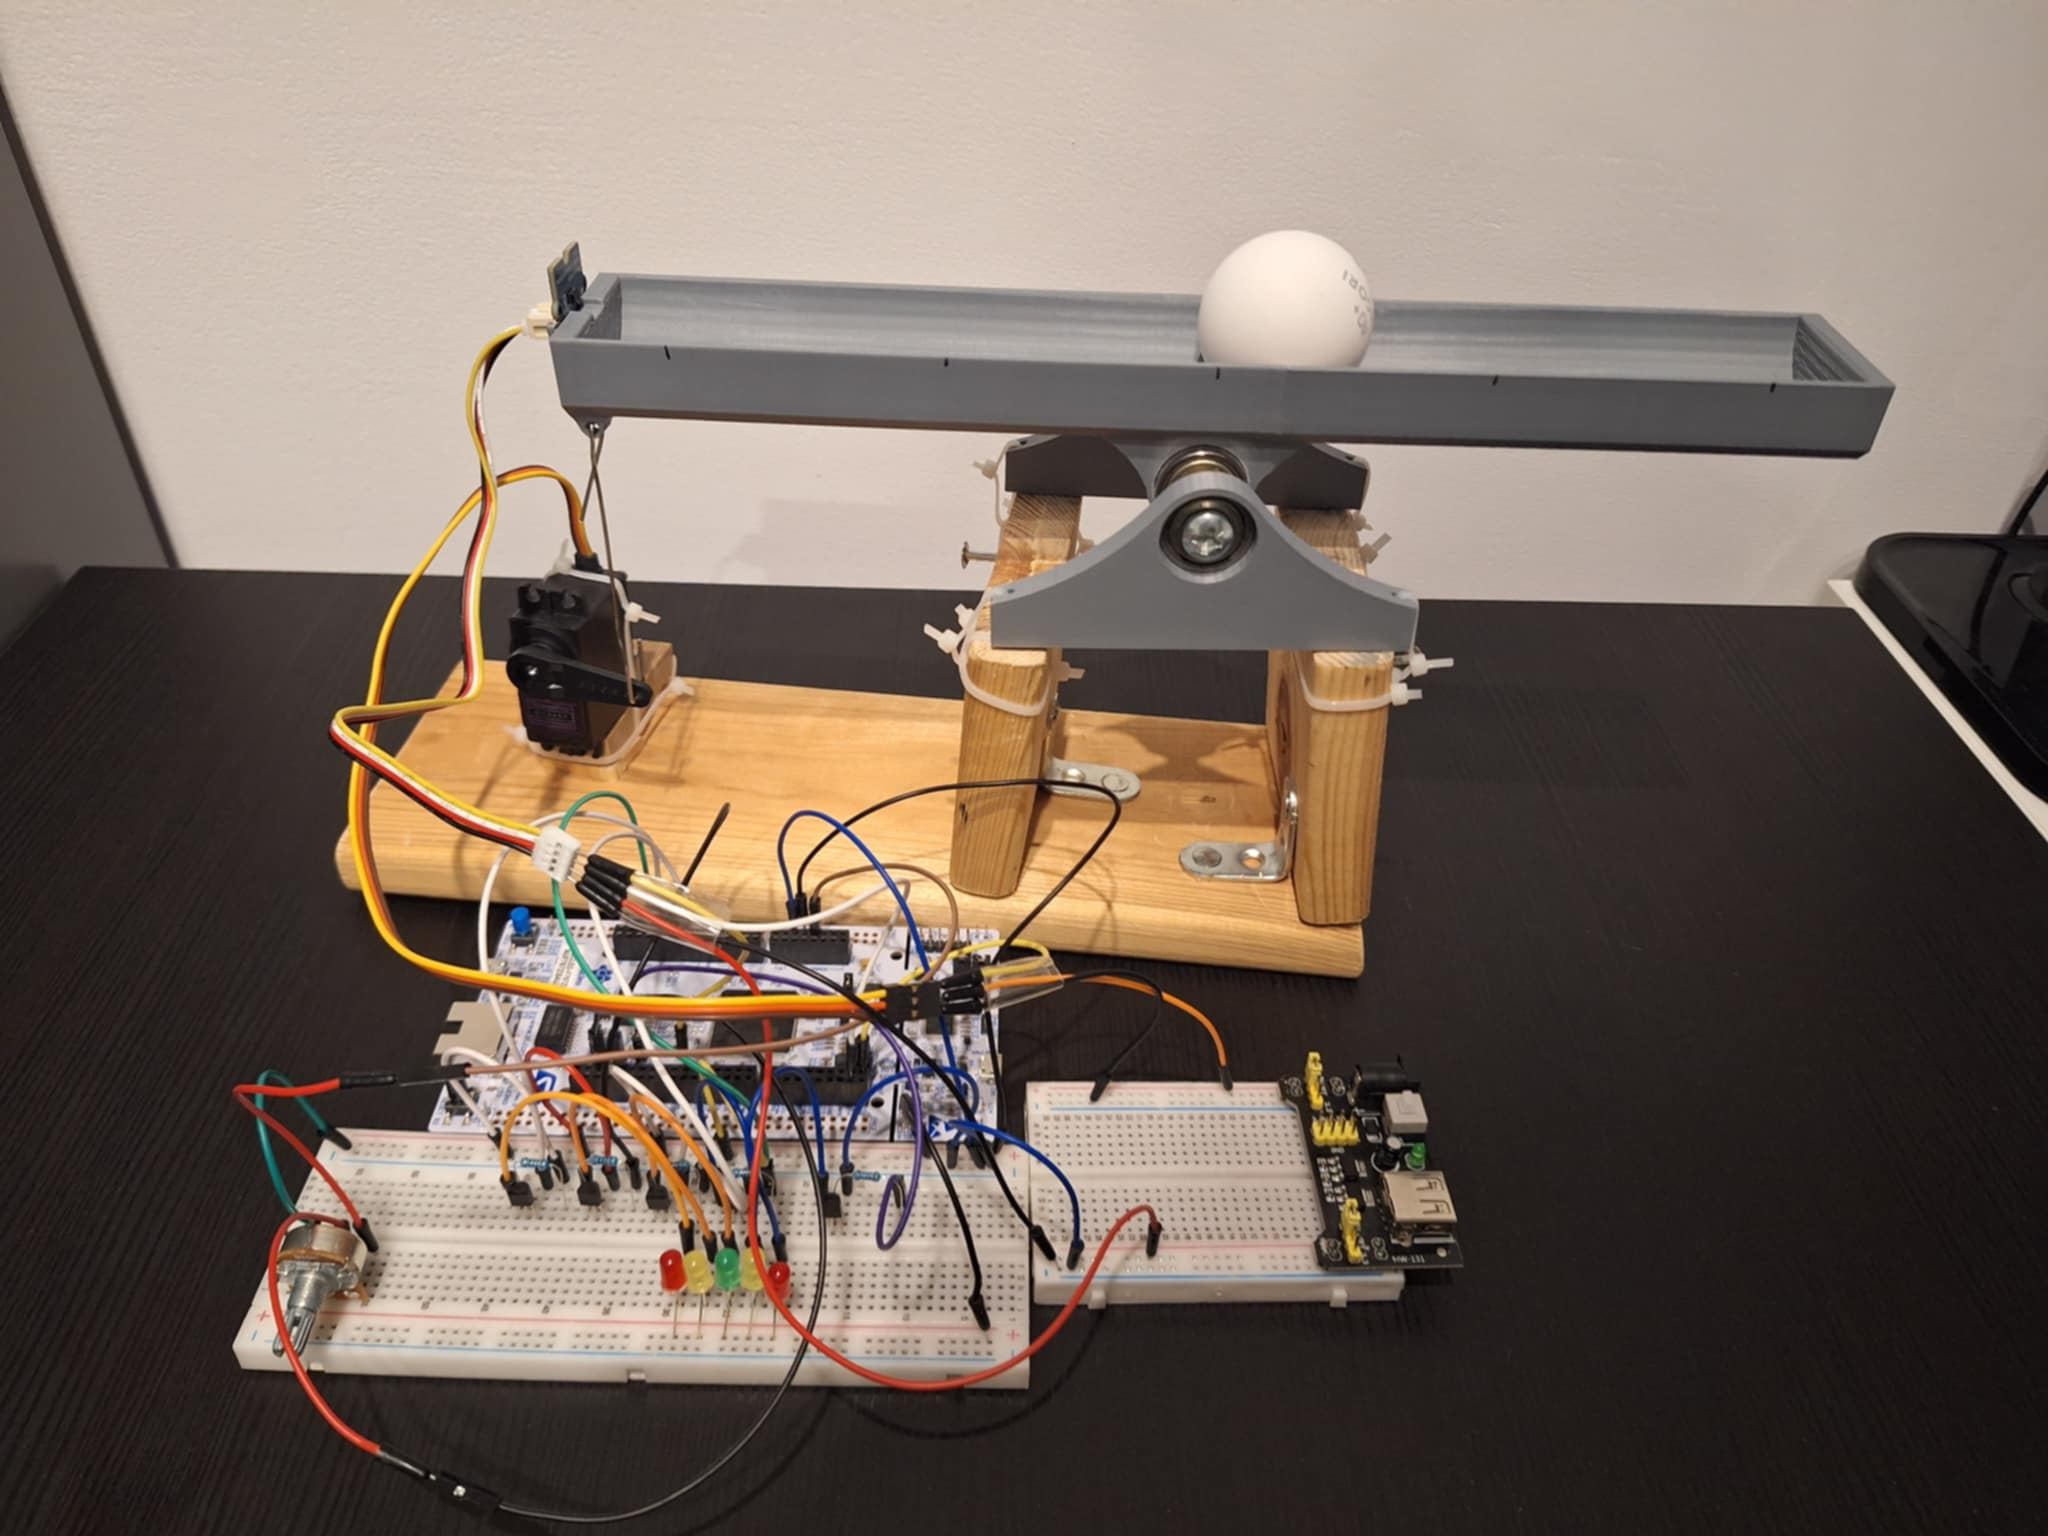
\includegraphics[width=0.8\linewidth]{2-budowa-stanowiska-i-oprogramowanie/2-img/stanowisko.png}
  \caption{Stanowisko laboratoryjne układu kulka na belce}
  \label{fig:stanowisko}
\end{figure}

\subsection{Wykaz komponentów}

\begin{table}[H]
  \centering
  \caption{Komponenty sprzętowe stanowiska}
  \label{tab:komponenty}
  \begin{tabular}{lll}
    \toprule
    \textbf{Element} & \textbf{Model / opis} & \textbf{Interfejs} \\
    \midrule
    Mikrokontroler & STM32 Nucleo F767ZI & --- \\
    Serwomechanek  & TowerPro MG946R      & PWM 50\,Hz \\
    Czujnik odległości & Grove VL53L0X ToF & I\textsuperscript{2}C \\
    Potencjometr   & liniowy & ADC (PA0) \\
    Zasilacz       & 5\,V DC & --- \\
    \bottomrule
  \end{tabular}
\end{table}

% -----------------------------------------------------------------------
\section{Mikrokontroler STM32 i peryferia}
% -----------------------------------------------------------------------

\subsection{Mikrokontroler STM32F767ZI}

Głównym procesorem stanowiska jest mikrokontroler STM32F767ZI~\cite{stm32f767zi}
zamontowany na płytce ewaluacyjnej Nucleo-F767ZI.
Układ oparty jest na rdzeniu ARM Cortex-M7 taktowanym z~częstotliwością 216\,MHz
i~wyposażony jest w~bogatą gamę peryferiów: kilka interfejsów I\textsuperscript{2}C
i UART, timery sprzętowe, przetwornik ADC oraz obsługę sygnałów PWM.

\begin{figure}[H]
  \centering
  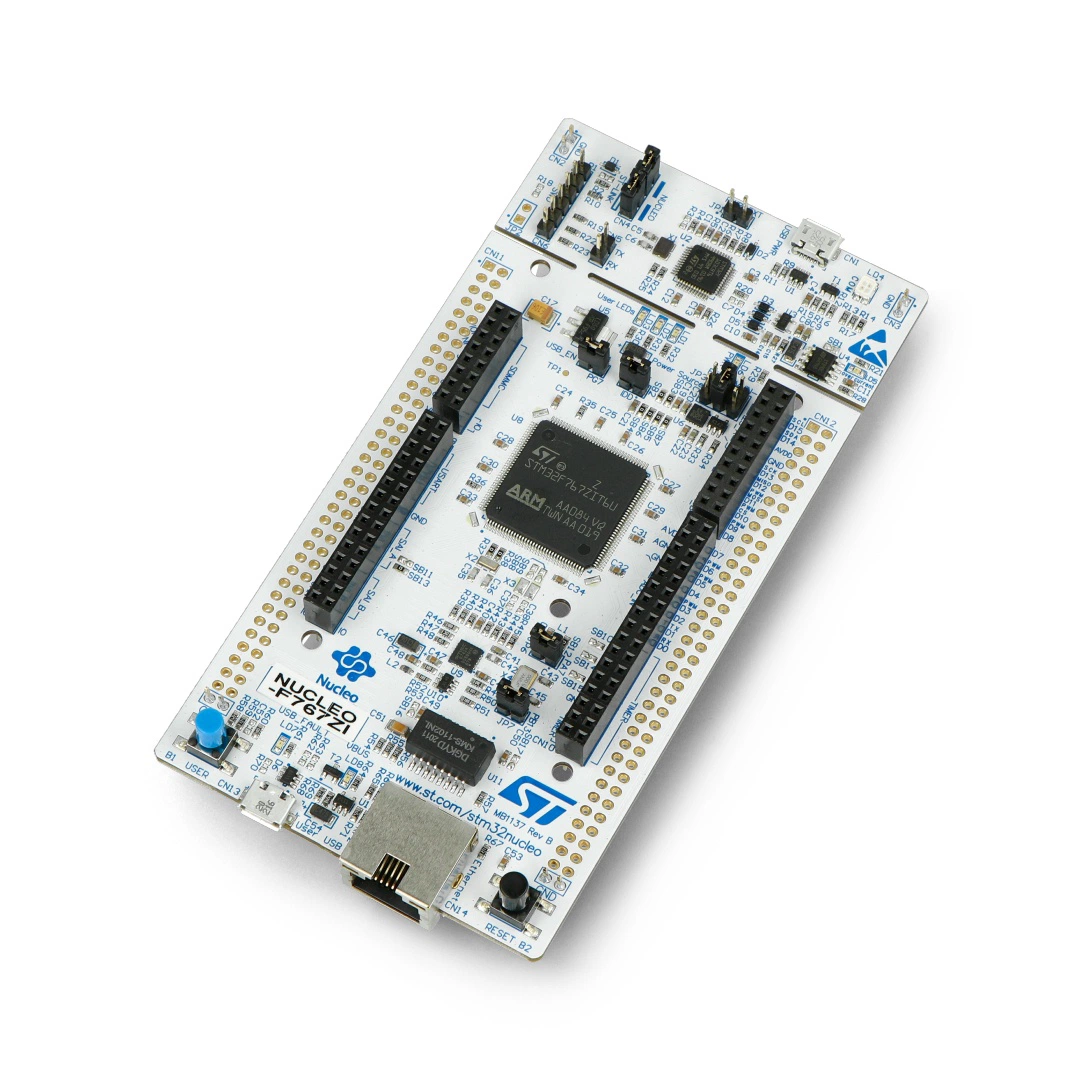
\includegraphics[width=0.45\linewidth]{2-budowa-stanowiska-i-oprogramowanie/2-img/plytka.png}
  \caption{Płytka ewaluacyjna STM32 Nucleo-F767ZI}
\end{figure}

\subsection{Serwomechanek MG946R}

Do sterowania kątem belki zastosowano serwomechanek TowerPro MG946R.
Serwo przyjmuje sygnał PWM o~częstotliwości 50\,Hz i~czasie wypełnienia
od 1\,ms (pełne wychylenie w~jedną stronę) do 2\,ms (pełne wychylenie
w~drugą stronę).
Zakres roboczy ograniczony jest w~oprogramowaniu do 60--140° w~celu
zabezpieczenia mechaniki.

\begin{figure}[H]
  \centering
  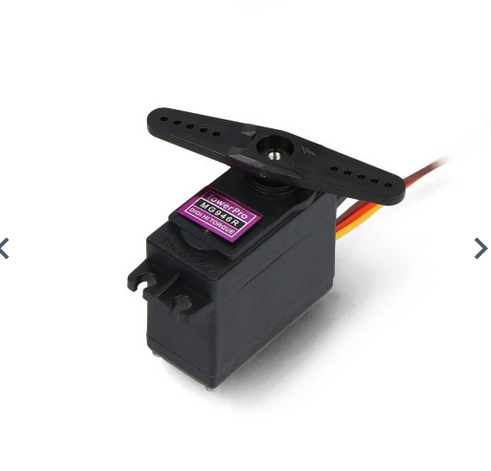
\includegraphics[width=0.35\linewidth]{2-budowa-stanowiska-i-oprogramowanie/2-img/servo.png}
  \caption{Serwomechanek TowerPro MG946R}
\end{figure}

\subsection{Czujnik odległości VL53L0X}

Pozycja kulki mierzona jest czujnikiem VL53L0X~\cite{vl53l0x} firmy
STMicroelectronics, pracującym w~technologii Time-of-Flight (ToF).
Czujnik emituje krótkie impulsy laserowe podczerwieni i~mierzy czas
powrotu odbitego sygnału, co pozwala wyznaczyć odległość z~rozdzielczością
1\,mm w~zakresie do 2\,m.
Komunikacja z~mikrokontrolerem odbywa się przez magistralę I\textsuperscript{2}C.

\begin{figure}[H]
  \centering
  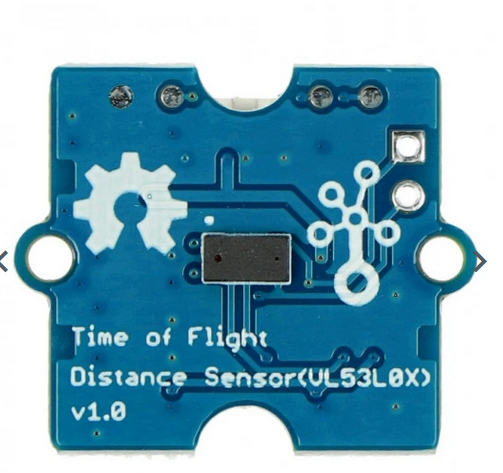
\includegraphics[width=0.4\linewidth]{2-budowa-stanowiska-i-oprogramowanie/2-img/sensor.png}
  \caption{Czujnik odległości Grove VL53L0X Time-of-Flight}
\end{figure}

\subsection{Potencjometr}

Potencjometr liniowy podłączony do wejścia analogowego PA0 (ADC1\_CH0)
umożliwia ręczne zadawanie wartości referencyjnej pozycji kulki
w~trybie analogowym.
Przetwornik ADC skonfigurowany jest z~rozdzielczością 12-bitową
($0$--$4095$), co odpowiada zakresowi pozycji $0$--$250\,\mathrm{mm}$.

% -----------------------------------------------------------------------
\section{Środowisko programistyczne}
% -----------------------------------------------------------------------

\subsection{Firmware STM32}

Oprogramowanie mikrokontrolera zostało opracowane w~środowisku
STM32CubeIDE (Eclipse CDT ze zintegrowanym kompilatorem ARM GCC).
Konfigurację peryferiów (timery, I\textsuperscript{2}C, UART, ADC, PWM)
wygenerowano za pomocą narzędzia STM32CubeMX.
Kod źródłowy podzielono na osobne moduły~C zgodnie ze standardem Doxygen:

\begin{table}[H]
  \centering
  \caption{Moduły firmware}
  \label{tab:moduly}
  \begin{tabular}{ll}
    \toprule
    \textbf{Moduł} & \textbf{Opis} \\
    \midrule
    \texttt{main.c/h}       & Główna aplikacja, konfiguracja peryferiów \\
    \texttt{servo\_pid.c/h} & Regulator PID z~anti-windup \\
    \texttt{lqr.c/h}        & Regulator LQR (przestrzeń stanów) \\
    \texttt{filters.c/h}    & Filtry cyfrowe (EMA, mediana, 1-Euro) \\
    \texttt{crc8.c/h}       & Suma kontrolna CRC-8 \\
    \texttt{calibration.c/h}& Kalibracja czujnika VL53L0X \\
    \texttt{vl53l0x.c/h}    & Sterownik czujnika (I\textsuperscript{2}C) \\
    \bottomrule
  \end{tabular}
\end{table}

System operacyjny czasu rzeczywistego FreeRTOS zarządza wykonaniem dwóch
wątków (tasków):
\begin{itemize}
  \item \texttt{ControlTask} (priorytet wysoki) — pętla sterowania;
  \item \texttt{DefaultTask} (priorytet normalny) — obsługa komend UART.
\end{itemize}

\subsection{Aplikacja desktopowa}

Aplikacja nadzorcza napisana jest w~języku Python~3 z~wykorzystaniem
frameworka PySide6 (Qt~6).
Zapewnia ona:
\begin{itemize}
  \item połączenie z~mikrokontrolerem przez port szeregowy (pyserial),
  \item wizualizację sygnałów w~czasie rzeczywistym (pyqtgraph),
  \item zadawanie wartości referencyjnej i~nastaw regulatorów,
  \item nagrywanie danych i~eksport do pliku CSV,
  \item podgląd kamery z~detekcją pozycji kulki (OpenCV).
\end{itemize}

\begin{figure}[H]
  \centering
  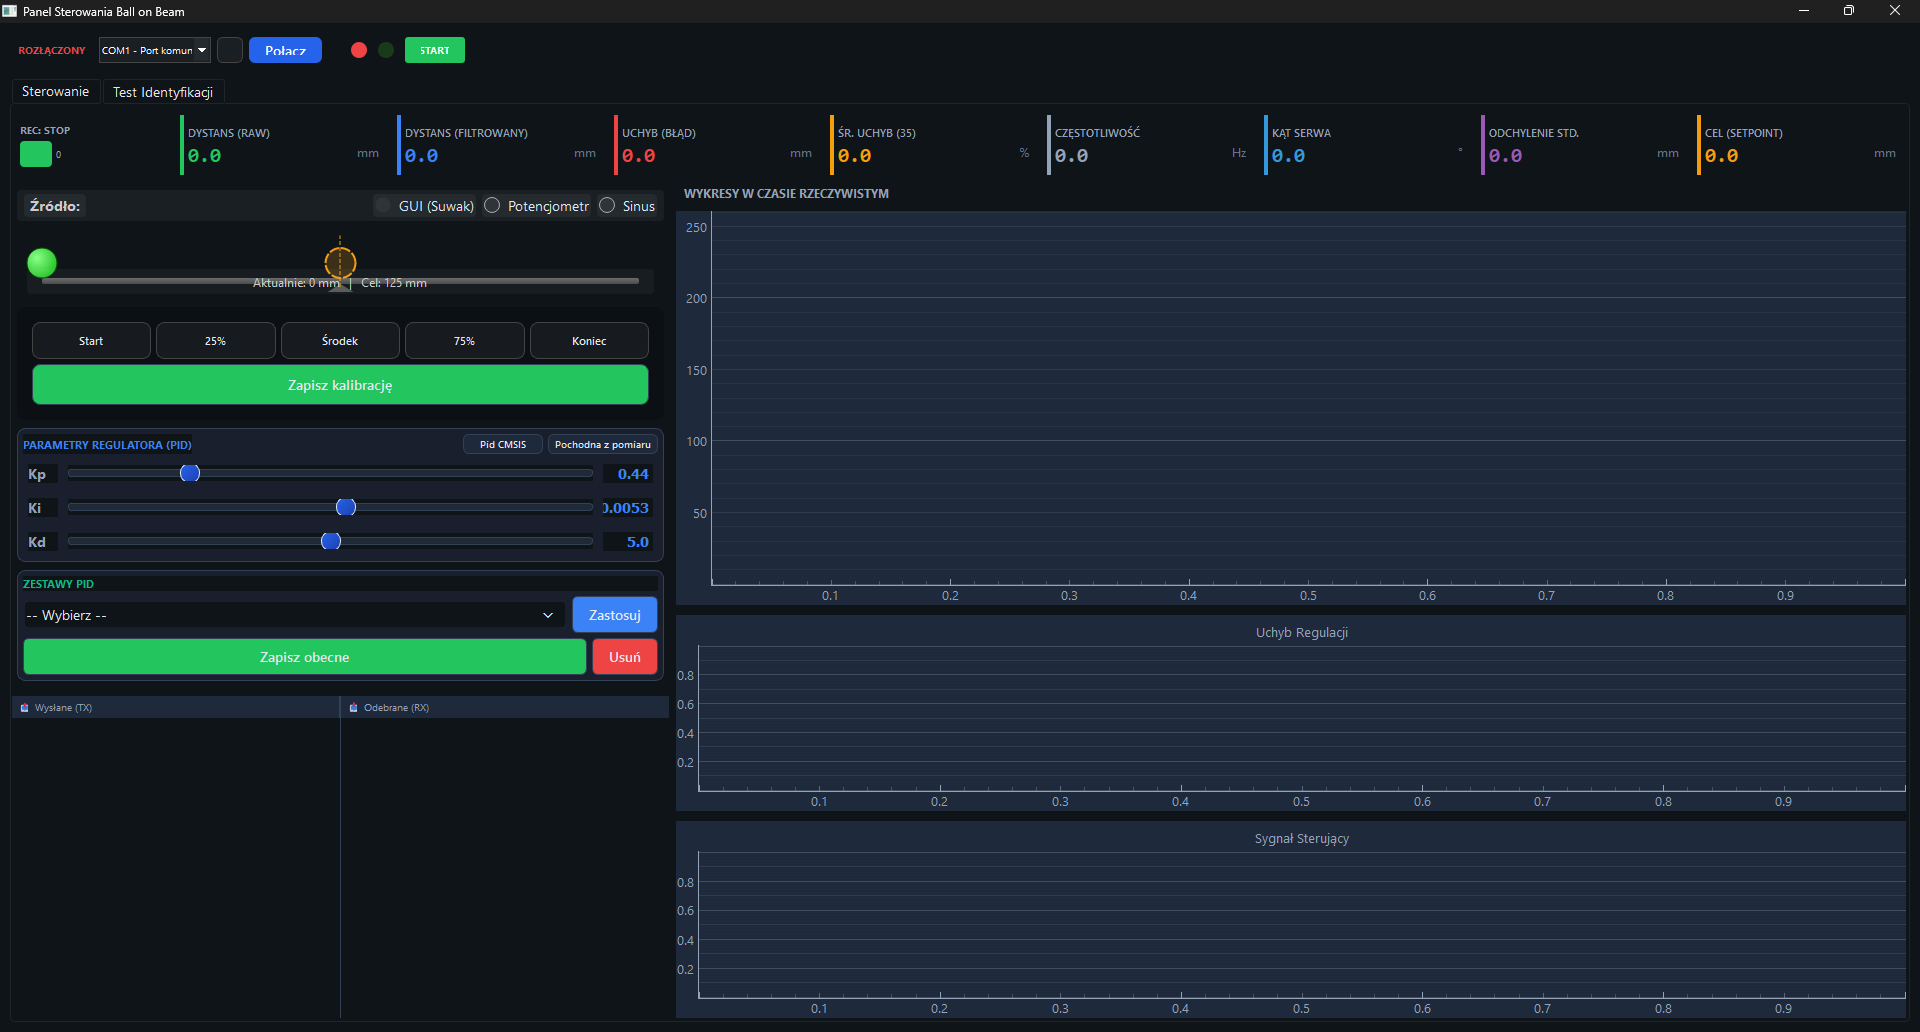
\includegraphics[width=0.9\linewidth]{2-budowa-stanowiska-i-oprogramowanie/2-img/desktop.png}
  \caption{Okno aplikacji desktopowej (PySide6)}
  \label{fig:desktop}
\end{figure}

% -----------------------------------------------------------------------
\section{Implementacja algorytmu sterowania}
% -----------------------------------------------------------------------

\subsection{Pętla sterowania i okres próbkowania}

Algorytm sterowania realizowany jest przez \texttt{ControlTask} z~ustalonym
okresem próbkowania 30\,ms wymuszonym przez funkcję \texttt{osDelay()}:

\begin{lstlisting}[style=cstyle, caption={Stały okres próbkowania w pętli sterowania (main.c)}]
#define PID_DT_MS 30

for (;;) {
    distance = readRangeContinuousMillimeters(&distanceStr);

    // obliczenia regulatora ...

    SetServoAngle(pid_output);
    osDelay(PID_DT_MS); // staly okres 30 ms
}
\end{lstlisting}

\subsection{Ograniczenie zakresu serwa}

Wyjście regulatora jest nasycane do bezpiecznego zakresu kąta serwa:

\begin{lstlisting}[style=cstyle, caption={Saturacja wyjścia i ograniczenia serwa (main.c)}]
#define SERVO_MIN_LIMIT  60.0f
#define SERVO_MAX_LIMIT 140.0f

if (pid_angle < SERVO_MIN_LIMIT)  pid_angle = SERVO_MIN_LIMIT;
if (pid_angle > SERVO_MAX_LIMIT)  pid_angle = SERVO_MAX_LIMIT;
SetServoAngle(pid_angle);
\end{lstlisting}

\subsection{Protokół telemetrii UART z sumą kontrolną CRC-8}

Dane pomiarowe przesyłane są przez UART~3 (115200\,baud) w~formacie
tekstowym z~sumą kontrolną CRC-8 (wielomian 0x07).
Format ramki:
\[
\texttt{D:\%d;Z:\%d;A:\%d;F:\%d;E:\%d;V:\%d;S:\%d;C:\%02X\textbackslash r\textbackslash n}
\]
gdzie kolejne pola oznaczają: surowy dystans, setpoint, kąt serwa,
dystans filtrowany, uchyb, średni uchyb, status czujnika i~CRC.

\begin{lstlisting}[style=cstyle, caption={Implementacja CRC-8 (crc8.c)}]
uint8_t CalculateCRC8(const char *data, int len) {
    uint8_t crc = 0x00;
    for (int i = 0; i < len; i++) {
        crc ^= data[i];
        for (uint8_t j = 0; j < 8; j++) {
            if (crc & 0x80)
                crc = (crc << 1) ^ 0x07;
            else
                crc <<= 1;
        }
    }
    return crc;
}
\end{lstlisting}

\subsection{Zadania FreeRTOS}

System operacyjny czasu rzeczywistego tworzy dwa wątki:

\begin{lstlisting}[style=cstyle, caption={Tworzenie zadań FreeRTOS (main.c)}]
osThreadDef(defaultTask, StartDefaultTask,
            osPriorityNormal, 0, 256);
defaultTaskHandle = osThreadCreate(osThread(defaultTask), NULL);

osThreadDef(ControlTask, StartControlTask,
            osPriorityHigh, 0, 1024);
ControlTaskHandle = osThreadCreate(osThread(ControlTask), NULL);

osKernelStart();
\end{lstlisting}

